\documentclass[12pt]{report}
\usepackage[utf8]{inputenc}
\usepackage[russian]{babel}
%\usepackage[14pt]{extsizes}
\usepackage{listings}
\usepackage{graphicx}
\usepackage{amsmath,amsfonts,amssymb,amsthm,mathtools} 
\usepackage{pgfplots}
\usepackage{filecontents}
\usepackage{float}
\usepackage{comment}
\usepackage{indentfirst}
\usepackage{eucal}
\usepackage{enumitem}
%s\documentclass[openany]{book}
\frenchspacing

\usepackage{array}

\usepackage{verbatim}

\usepackage{caption}
\captionsetup{labelsep=endash}
\captionsetup[figure]{name={Рисунок}}

\usepackage{indentfirst} % Красная строка

\usetikzlibrary{datavisualization}
\usetikzlibrary{datavisualization.formats.functions}

\usepackage{amsmath}


% Для листинга кода:
\lstset{ %
	language=c,                 % выбор языка для подсветки (здесь это С)
	basicstyle=\small\sffamily, % размер и начертание шрифта для подсветки кода
	numbers=left,               % где поставить нумерацию строк (слева\справа)
	numberstyle=\tiny,           % размер шрифта для номеров строк
	stepnumber=1,                   % размер шага между двумя номерами строк
	numbersep=5pt,                % как далеко отстоят номера строк от подсвечиваемого кода
	showspaces=false,            % показывать или нет пробелы специальными отступами
	showstringspaces=false,      % показывать или нет пробелы в строках
	showtabs=false,             % показывать или нет табуляцию в строках
	frame=single,              % рисовать рамку вокруг кода
	tabsize=2,                 % размер табуляции по умолчанию равен 2 пробелам
	captionpos=t,              % позиция заголовка вверху [t] или внизу [b] 
	breaklines=true,           % автоматически переносить строки (да\нет)
	breakatwhitespace=false, % переносить строки только если есть пробел
	escapeinside={\#*}{*)}   % если нужно добавить комментарии в коде
}


\usepackage[left=2cm,right=2cm, top=2cm,bottom=2cm,bindingoffset=0cm]{geometry}
% Для измененных титулов глав:
\usepackage{titlesec, blindtext, color} % подключаем нужные пакеты
\definecolor{gray75}{gray}{0.75} % определяем цвет
\newcommand{\hsp}{\hspace{20pt}} % длина линии в 20pt
% titleformat определяет стиль
\titleformat{\chapter}[hang]{\Huge\bfseries}{\thechapter\hsp\textcolor{gray75}{|}\hsp}{0pt}{\Huge\bfseries}


% plot
\usepackage{pgfplots}
\usepackage{filecontents}
\usetikzlibrary{datavisualization}
\usetikzlibrary{datavisualization.formats.functions}

\begin{document}
	%\def\chaptername{} % убирает "Глава"
	\thispagestyle{empty}
	\begin{titlepage}
		\noindent \begin{minipage}{0.15\textwidth}
			
\includegraphics[width=\linewidth]{inc/b_logo}
		\end{minipage}
		\noindent\begin{minipage}{0.9\textwidth}\centering
			\textbf{Министерство науки и высшего образования Российской Федерации}\\
			\textbf{Федеральное государственное бюджетное образовательное учреждение высшего образования}\\
			\textbf{~~~«Московский государственный технический университет имени Н.Э.~Баумана}\\
			\textbf{(национальный исследовательский университет)»}\\
			\textbf{(МГТУ им. Н.Э.~Баумана)}
		\end{minipage}
		
		\noindent\rule{18cm}{3pt}
		\newline\newline
		\noindent ФАКУЛЬТЕТ $\underline{\text{«Информатика и системы управления»}}$ \newline\newline
		\noindent КАФЕДРА $\underline{\text{«Программное обеспечение ЭВМ и информационные технологии»}}$\newline\newline\newline\newline\newline
		
		\begin{center}
			\noindent\begin{minipage}{1.1\textwidth}\centering
				\Large\textbf{Отчет по лабораторной работе №4}\newline
				\textbf{по дисциплине <<Моделирование>>}\newline\newline
			\end{minipage}
		\end{center}
		
		\noindent\textbf{Тема} $\underline{\text{Алгоритмы продвижения модельного времени}}$\newline\newline
		\noindent\textbf{Студент} $\underline{\text{Слепокурова М.Ф.}}$\newline\newline
		\noindent\textbf{Группа} $\underline{\text{ИУ7-76Б}}$\newline\newline
		\noindent\textbf{Оценка (баллы)} $\underline{\text{~~~~~~~~~~~~~~~~~}}$\newline\newline
		\noindent\textbf{Преподаватель} $\underline{\text{Рудаков И.В.}}$\newline\newline\newline
		
		\begin{center}
			\vfill
			Москва~---~\the\year
			~г.
		\end{center}
	\end{titlepage}

\setcounter{page} {2}





\section*{Постановка задачи}
Промоделировать систему, состоящую из источника информации (ИИ), буферной памяти (БП) и обслуживающего аппарата (ОА), используя принцип $\Delta t$ и событийный алгоритм. Источник информации генерирует заявки, время появления которых распределено по равномерному закону, а обслуживающий аппарат обрабатывает каждую из них за время, распределенное по закону Эрланга.
Определить минимальный размер буферной памяти, при которой не будет потерь заявок. Учесть возможность задания вероятности повторного попадания заявок из обслуживающего аппарата в очередь.


\section*{Теория}
\subsection*{Принцип $\Delta t$}
Данный принцип заключается в последовательном анализе состояний всех блоков в момент $t + \Delta t$ по заданному состоянию блоков в момент времени $t$, при этом новое состояние блоков определяется в соответствии с их алгоритмическим описанием с учетом действующих случайных факторов, задаваемых распределениями вероятности. В результате такого анализа принимается решение о том, какие общесистемные события должны имитироваться программной моделью на данный момент времени.

Основной недостаток принципа --- значительные затраты вычислительных ресурсов, а при недостаточно малом $\Delta t$ появляется опасность пропуска отдельных событий в системе, исключающая возможность получения правильных результатов при моделировании.

К достоинствам метода можно отнести равномерную протяжку модельного времени в виду фиксированного временного интервала $\Delta t$.

\subsection*{Событийный принцип}
Характерное свойство систем обработки информации заключается в том, что состояния отдельных устройств изменяются в дискретные моменты времени, совпадающие с моментами времени поступления сообщений в систему, окончания реализации процесса, возникновения прерываний и аварийных сигналов и т.д. Поэтому моделирование и продвижение времени в системе удобно проводить, используя событийный принцип, при котором состояние всех блоков имитационной модели анализируется лишь в момент появления какого-либо события. Момент поступления следующего события определяется минимальным значением из списка будущих событий, представляющего собой совокупность моментов ближайшего изменения состояния каждого из блоков системы.


\subsection*{Равномерное распределение}
Равномерное распределение описывает случайную величину, принимающую значения, принадлежащие некоторому промежутку конечной длины, при этом плотность вероятности в этом промежутке всюду постоянна.
\newline

Функция распределения равномерной непрерывной случайной величины имеет следующий вид:
\begin{equation*}
	F(x) = \begin{cases}
		0, & x \leq a \\
		\frac{x-a}{b-a}, & a \leq x \leq b \\
		1, & x > b
	\end{cases}
\end{equation*}

Плотность распределения равномерной непрерывной случайной величины имеет следующий вид:
\begin{equation*}
	f(x) = \begin{cases}
		\frac{1}{b-a}, & a \leq x \leq b \\
		0, & \text{иначе}
	\end{cases}
\end{equation*}

В качестве параметров по умолчанию для равномерного распределения использовались значения $a = 1$ и $b = 10$.

\subsection*{Распределение Эрланга}
Распределение Эрланга описывает непрерывную случайную величину, принимающую неотрицательные значения и представляющую собой сумму $n$ независимых случайных величин, распределенных по одному и тому же экспоненциальному закону с параметром $\lambda$.
\newline

Функция распределения Эрланга непрерывной случайной величины имеет следующий вид:
\begin{equation*}
	F(x) = 1 - e^{-x/\lambda} \sum_{i=0}^{n-1} \frac{(x/\lambda)^i}{i!} 
\end{equation*}

Плотность распределения Эрланга непрерывной случайной величины имеет следующий вид:
\begin{equation*}
	f(x) = \frac{x^{n-1}e^{-x\lambda}\lambda^n}{(n-1)!}
\end{equation*}

В качестве параметров по умолчанию для распределения Эрланга использовались значения $n = 9$ и $\lambda = 0.5$.

\section*{Средства реализации}

Для реализации приложения был выбран язык программирования Python.

\clearpage
\section*{Листинг кода}

\begin{lstlisting}
class RequestGenerator:
  def __init__(self, generator):
    self._generator = generator
    self._receivers = set()

  def addReceiver(self, receiver):
    self._receivers.add(receiver)

  def removeReceiver(self, receiver):
    if (receiver in self._receivers):
      self._receivers.remove(receiver)

  def nextTimePeriod(self):
    return self._generator.generateTime()

  def emitRequest(self):
    for receiver in self._receivers:
      receiver.receiveRequest()
      
class RequestProcessor():
  def __init__(self, generator, reenterProbability=0):
    self._generator = generator
    self._currQueueSize = 0
    self._maxQueueSize = 0
    self._processedRequests = 0
    self._reenterProbability = reenterProbability
    self._reenteredRequests = 0

  def processedRequests(self):
    return self._processedRequests

  def maxQueueSize(self):
    return self._maxQueueSize

  def currQueueSize(self):
    return self._currQueueSize

  def reenteredRequests(self):
    return self._reenteredRequests

  def process(self):
    if self._currQueueSize > 0:
      self._processedRequests += 1
      self._currQueueSize -= 1
      if nr.random_sample() < self._reenterProbability:
        self._reenteredRequests += 1
\end{lstlisting}
\clearpage
\begin{lstlisting}
        self.receiveRequest()

  def receiveRequest(self):
    self._currQueueSize += 1
    if self._currQueueSize > self._maxQueueSize:
      self._maxQueueSize += 1

  def nextTimePeriod(self):
    return self._generator.generateTime()

class Modeller:
  def __init__(self, generator, processor):
    self._generator = generator
    self._processor = processor
    self._generator.addReceiver(self._processor)

  def eventBasedModelling(self, requestCount):
    generator = self._generator
    processor = self._processor

    genPeriod = generator.nextTimePeriod()
    procPeriod = genPeriod + processor.nextTimePeriod()
    while processor.processedRequests() < requestCount:
      if genPeriod <= procPeriod:
        generator.emitRequest()
        genPeriod += generator.nextTimePeriod()
      else:
        processor.process()
        if processor.currQueueSize() > 0:
          procPeriod += processor.nextTimePeriod()
        else:
          procPeriod = genPeriod + processor.nextTimePeriod()

    return { "processedRequests": processor.processedRequests(),
             "reenteredRequests": processor.reenteredRequests(),
             "maxQueueSize": processor.maxQueueSize() }

  def timeBasedModelling(self, requestCount, dt=1):
    generator = self._generator
    processor = self._processor

    genPeriod = generator.nextTimePeriod()
    procPeriod = genPeriod + processor.nextTimePeriod()
    currTime = 0
    while processor.processedRequests() < requestCount:
      if genPeriod <= currTime:
        generator.emitRequest()
        genPeriod += generator.nextTimePeriod()
      if procPeriod <= currTime:
\end{lstlisting}
\clearpage
\begin{lstlisting}
        processor.process()
        if processor.currQueueSize() > 0:
          procPeriod += processor.nextTimePeriod()
        else:
          procPeriod = genPeriod + processor.nextTimePeriod()
      currTime += dt

    return { "processedRequests": processor.processedRequests(),
             "reenteredRequests": processor.reenteredRequests(),
             "maxQueueSize": processor.maxQueueSize() }

generator = RequestGenerator(UniformGenerator())
processor = RequestProcessor(ErlangGenerator(), REENTER_PROBABILITY)
model = Modeller(generator, processor)
resultTimeBased = model.timeBasedModelling(REQUEST_COUNT, DELTA_T)
print("Time algorithm:")
print("-" * 26)
print("Processed requests: ", resultTimeBased["processedRequests"])
print("Reenter probability: ", REENTER_PROBABILITY)
print("Reentered requests: ", resultTimeBased["reenteredRequests"])
print("Buffer memory size: ", resultTimeBased["maxQueueSize"])
print("\n")

generator = RequestGenerator(UniformGenerator())
processor = RequestProcessor(ErlangGenerator(), REENTER_PROBABILITY)
model = Modeller(generator, processor)
resultEventBased = model.eventBasedModelling(REQUEST_COUNT)
print("Event algorithm:")
print("-" * 26)
print("Processed requests: ", resultEventBased["processedRequests"])
print("Reenter probability: ", REENTER_PROBABILITY)
print("Reentered requests: ", resultEventBased["reenteredRequests"])
print("Buffer memory size: ", resultEventBased["maxQueueSize"])
\end{lstlisting}


\clearpage
\section*{Демонстрация работы программы}
На рисунке \ref{fig:pic1} изображен пример работы программы для 10000 заявок с вероятностью повторного попадания заявки в очередь = 0.

\begin{figure}[h!btp]
	\centering
	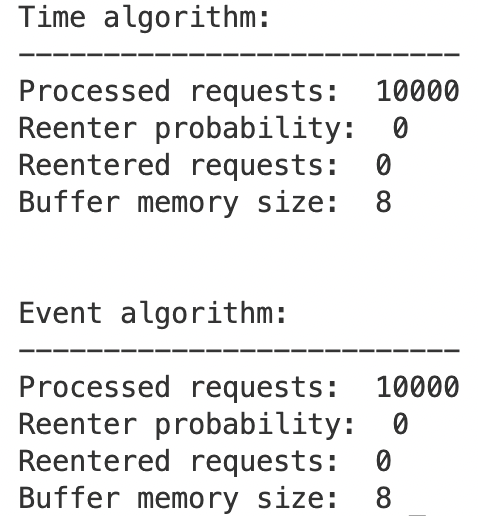
\includegraphics[width=0.4\textwidth]{inc/pic1.png}
	\caption{Пример работы программы --- 1}
	\label{fig:pic1}	
\end{figure}

На рисунке \ref{fig:pic2} изображен пример работы программы для 10000 заявок с вероятностью повторного попадания заявки в очередь = 0.1.

\begin{figure}[h!btp]
	\centering
	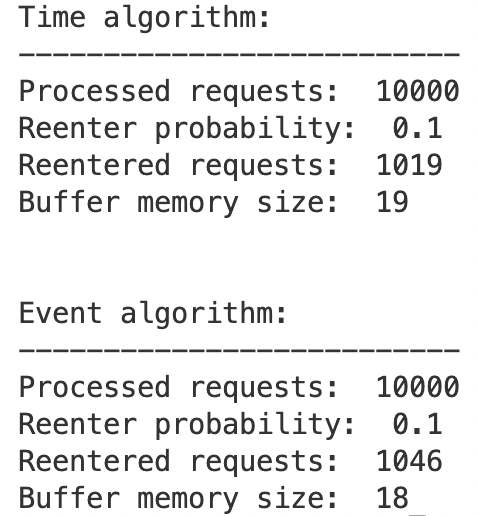
\includegraphics[width=0.4\textwidth]{inc/pic2.png}
	\caption{Пример работы программы --- 2}
	\label{fig:pic2}	
\end{figure}
\clearpage

На рисунке \ref{fig:pic3} изображен пример работы программы для 10000 заявок с вероятностью повторного попадания заявки в очередь = 0.3.

\begin{figure}[h!btp]
	\centering
	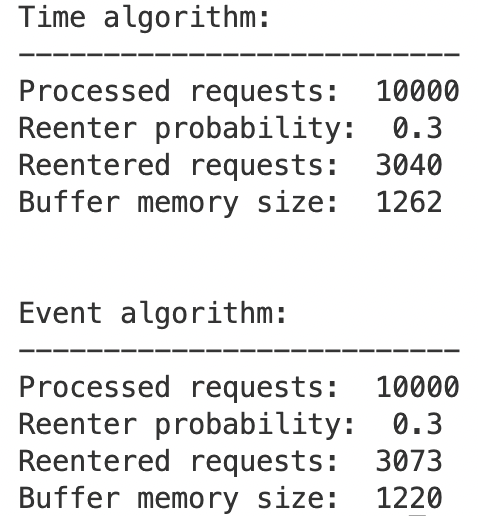
\includegraphics[width=0.4\textwidth]{inc/pic3.png}
	\caption{Пример работы программы --- 3}
	\label{fig:pic3}	
\end{figure}

На рисунке \ref{fig:pic4} изображен пример работы программы для 10000 заявок с вероятностью повторного попадания заявки в очередь = 0.5.

\begin{figure}[h!btp]
	\centering
	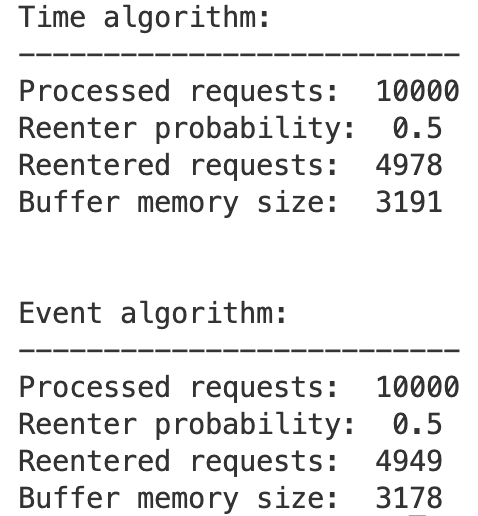
\includegraphics[width=0.4\textwidth]{inc/pic4.png}
	\caption{Пример работы программы --- 4}
	\label{fig:pic4}	
\end{figure}
\clearpage

На рисунке \ref{fig:pic5} изображен пример работы программы для 10000 заявок с вероятностью повторного попадания заявки в очередь = 0.7.

\begin{figure}[h!btp]
	\centering
	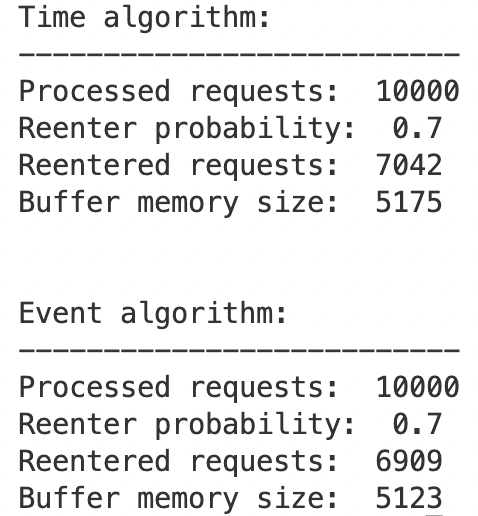
\includegraphics[width=0.4\textwidth]{inc/pic5.png}
	\caption{Пример работы программы --- 5}
	\label{fig:pic5}	
\end{figure}

На рисунке \ref{fig:pic6} изображен пример работы программы для 10000 заявок с вероятностью повторного попадания заявки в очередь = 1.

\begin{figure}[h!btp]
	\centering
	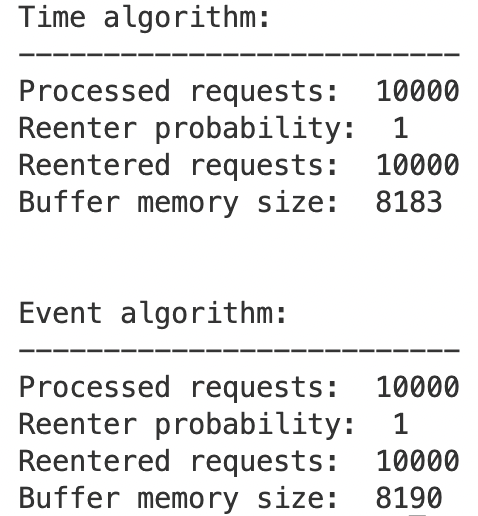
\includegraphics[width=0.4\textwidth]{inc/pic6.png}
	\caption{Пример работы программы --- 6}
	\label{fig:pic6}	
\end{figure}

\bibliographystyle{utf8gost705u}  % стилевой файл для оформления по ГОСТу
\bibliography{51-biblio}          % имя библиографической базы (bib-файла)
	
\end{document}
